\chapter{Transistor BJT (Bipolar Junction Transistor)}
\label{ch:bjt}
\section{Amplificatore di Tensione a Emettitore Comune}

\begin{definizione}{Transistor Bipolare a Giunzione (BJT)}
    Il BJT è un dispositivo a semiconduttore caratterizzato da due giunzioni interagenti (Base-Emettitore e Base-Collettore). Per garantirne il corretto funzionamento e l'effetto transistor, esso presenta due proprietà costruttive fondamentali:
    \begin{itemize}[label=$\cdot$, leftmargin=*]
        \item La regione di base è progettata per essere fisicamente molto più stretta rispetto alle regioni di collettore ed emettitore.
        \item Il livello di drogaggio dell'emettitore è marcatamente superiore a quello del collettore.
    \end{itemize}
\end{definizione}

\begin{figure}[H]
    \centering
    \begin{circuitikz}[american, scale=1.0, transform shape]
        % Sorgente e accoppiamento
        \draw (0,2) to[V, l=$V_S$] (0,-1) node[ground]{};
        \draw (0,2) to[C, l=$C_{in}$] (2,2);
        % Partitore di base R1-R2
        \draw (2,5.5) to[R, l=$R_1$] (2,2) to[R, l=$R_2$] (2,-1) node[ground]{};
        \draw (2,5.5) -- (4.5,5.5) node[above]{$+V_{CC}$};
        % BJT npn
        \draw (4.5,2) node[npn, anchor=base](Q){$Q$};
        \draw (2,2) -- (Q.base);
        % RC e RE ortogonali
        \draw (Q.collector) to[R, l=$R_C$] (Q.collector |- 0,5.5) -- (2,5.5);
        \draw (Q.emitter)   to[R, l=$R_E$] (Q.emitter |- 0,-1) node[ground]{};
        % Disaccoppiamento uscita
        \draw (Q.collector) to[short, *-] ++(0.5,0) to[C, l=$C_{out}$] ++(2,0) node[right]{$V_{out}$};
    \end{circuitikz}
    \caption{Schema dell'amplificatore BJT a emettitore comune. Il partitore $R_1$--$R_2$ fissa la tensione di base e quindi il punto di lavoro (polarizzazione a partitore). $R_C$ è la resistenza di carico al collettore; $R_E$ introduce la degenerazione d'emettitore che migliora la stabilità termica. I condensatori $C_{in}$ e $C_{out}$ disaccoppiano la componente continua dal segnale.}
\end{figure}

\begin{figure}[H]
    \centering
    \begin{circuitikz}[american, scale=1.1, transform shape]
        % --- npn ---
        \draw (-2.5,0) node[npn](Q1){};
        \draw (Q1.C) -- ++(0,0.5) node[above] {C (Collettore)};
        \draw (Q1.E) -- ++(0,-0.5) node[below] {E (Emettitore)};
        \draw (Q1.B) -- ++(-0.5,0) node[left] {B (Base)};
        \node[font=\large] at (-2.5, -2) {\textbf{npn}};

        % --- pnp ---
        \draw (2.5,0) node[pnp](Q2){};
        \draw (Q2.E) -- ++(0,0.5) node[above] {E (Emettitore)};
        \draw (Q2.C) -- ++(0,-0.5) node[below] {C (Collettore)};
        \draw (Q2.B) -- ++(-0.5,0) node[left] {B (Base)};
        \node[font=\large] at (2.5, -2) {\textbf{pnp}};
    \end{circuitikz}
    \caption{Simboli circuitali del BJT npn (sinistra) e pnp (destra). Nel npn la freccia all'emettitore punta verso l'esterno (convenzione: direzione della corrente); nel pnp punta verso il transistor.}
\end{figure}

\subsubsection{Diagrammi a Bande di Energia (Qualitativi)}
\begin{osservazione}{Diagrammi a Bande di Energia (Qualitativi)}
    Il principio di funzionamento del BJT può essere compreso intuitivamente analizzando l'andamento delle barriere di potenziale che si instaurano tra i tre semiconduttori diversamente drogati.
    
    \vspace{0.2cm}
    \textbf{1. BJT all'Equilibrio (Nessun Generatore Esterno)} \\
    In assenza di polarizzazione, presso le giunzioni B--E e B--C si formano naturalmente due barriere di potenziale per gli elettroni (provenienti rispettivamente dall'emettitore e dal collettore). Il sistema si trova in uno stato di equilibrio termodinamico e non si osserva alcun passaggio di corrente netta.
    
    \vspace{0.3cm}
    \begin{center}
    \begin{tikzpicture}[scale=1.2, transform shape]
        % Axes
        \draw[->, thick] (0,0) -- (5.5,0) node[right, font=\small] {$x$};
        \draw[->, thick] (0,0) -- (0,2.6) node[above, font=\small] {$V(x)$};
        
        % Regions dividers
        \draw[dashed, color=gray!70] (1.8, 0) -- (1.8, 2.3);
        \draw[dashed, color=gray!70] (3.6, 0) -- (3.6, 2.3);
        
        % Regions labels
        \node[font=\small\bfseries] at (0.9, -0.35) {E (N)};
        \node[font=\small\bfseries] at (2.7, -0.35) {B (P)};
        \node[font=\small\bfseries] at (4.5, -0.35) {C (N)};
        
        % Base potential extension line for clear height measurement
        \draw[dotted, color=gray!60] (0.3, 0.5) -- (5.1, 0.5);

        % Potential curve
        \draw[very thick, color=noteteal] (0.3, 1.9) 
            -- (1.4, 1.9)
            .. controls (1.7, 1.9) and (1.7, 0.5) .. (2.0, 0.5)
            -- (3.4, 0.5) 
            .. controls (3.7, 0.5) and (3.7, 1.9) .. (4.0, 1.9)
            -- (5.1, 1.9);
            
        % Annotations (positioned clearly off the curve with background fill)
        \draw[<->, >=stealth, font=\footnotesize] (0.8, 0.5) -- (0.8, 1.9) node[midway, fill=white, inner sep=1.5pt] {$V_{\gamma,E}$};
        \draw[<->, >=stealth, font=\footnotesize] (4.6, 0.5) -- (4.6, 1.9) node[midway, fill=white, inner sep=1.5pt] {$V_{\gamma,C}$};
    \end{tikzpicture}
    \end{center}
    \vspace{0.4cm}
    
    \textbf{2. BJT Polarizzato in Zona Attiva (B--E in PD, B--C in PI)} \\
    In questa configurazione, l'applicazione di una tensione diretta abbassa significativamente la barriera B--E, consentendo una iniezione massiccia di elettroni dall'emettitore verso la base. Poiché la regione di base è estremamente sottile rispetto alla lunghezza di diffusione ($W_B \ll L_n$), la stragrande maggioranza degli elettroni riesce ad attraversarla senza subire ricombinazione e viene \emph{raccolta} dal collettore (grazie al campo elettrico favorevole generato dalla barriera B--C in polarizzazione inversa). Solo una minima frazione $(1-\alpha_F)$ di elettroni si ricombina con le lacune presenti in base, originando così una corrente di base $I_B$ molto ridotta rispetto a $I_C$ e $I_E$.

    \vspace{0.3cm}
    \begin{center}
    \begin{tikzpicture}[scale=1.2, transform shape]
        % Axes
        \draw[->, thick] (0,0) -- (5.5,0) node[right, font=\small] {$x$};
        \draw[->, thick] (0,0) -- (0,2.8) node[above, font=\small] {$V(x)$};
        
        % Regions dividers
        \draw[dashed, color=gray!70] (1.8, 0) -- (1.8, 2.5);
        \draw[dashed, color=gray!70] (3.6, 0) -- (3.6, 2.5);
        
        % Regions labels
        \node[font=\small\bfseries] at (0.9, -0.35) {E (N)};
        \node[font=\small\bfseries] at (2.7, -0.35) {B (P)};
        \node[font=\small\bfseries] at (4.5, -0.35) {C (N)};
        
        % Base potential extension line for height measurement
        \draw[dotted, color=gray!60] (0.3, 0.5) -- (5.1, 0.5);

        % Potential curve
        \draw[very thick, color=noteteal] (0.3, 1.1) 
            -- (1.4, 1.1)
            .. controls (1.7, 1.1) and (1.7, 0.5) .. (2.0, 0.5)
            -- (3.4, 0.5) 
            .. controls (3.7, 0.5) and (3.7, 2.4) .. (4.0, 2.4)
            -- (5.1, 2.4);
            
        % Annotations (positioned cleanly with fill=white)
        \draw[<->, >=stealth, font=\footnotesize] (0.8, 0.5) -- (0.8, 1.1) node[midway, fill=white, inner sep=1.5pt] {$V_{\gamma} - V_{BE}$};
        \draw[<->, >=stealth, font=\footnotesize] (4.6, 0.5) -- (4.6, 2.4) node[midway, fill=white, inner sep=1.5pt] {$V_{\gamma} + |V_{BC}|$};
    \end{tikzpicture}
    \end{center}
    
    \vspace{0.2cm}
    Dal punto di vista macroscopico, le correnti si legano tramite le seguenti relazioni lineari:
    \[
        I_C = \alpha_F\,I_E,
        \qquad
        I_B = (1-\alpha_F)\,I_E,
        \qquad
        \alpha_F \in [0.99,\,0.995]
    \]
\end{osservazione}

\subsubsection{Equazioni di Ebers-Moll}
\begin{teorema}{Modello di Ebers-Moll}
    Il modello matematico completo che descrive il comportamento macroscopico del BJT combina il Principio di Kirchhoff sui nodi con le equazioni di Shockley modificate per ciascuna giunzione. Tali equazioni costituiscono il sistema di Ebers-Moll \cite{sedra}:
    \begin{align}
        I_C + I_B + I_E &= 0 \tag{KCL}\\
        I_E &= -I_{ES}\!\left[e^{V_{BE}/(mV_T)}-1\right]
             + \alpha_R I_{CS}\!\left[e^{V_{BC}/(mV_T)}-1\right] \tag{E--M Emit.}\\
        I_C &= -I_{CS}\!\left[e^{V_{BC}/(mV_T)}-1\right]
             + \alpha_F I_{ES}\!\left[e^{V_{BE}/(mV_T)}-1\right] \tag{E--M Coll.}
    \end{align}
    
    I parametri chiave del modello assumono i seguenti significati fisici:
    \begin{center}
    \begin{adjustbox}{max width=\textwidth}
    \renewcommand{\arraystretch}{1.2}
    \begin{tabular}{cll}
        \hline
        \textbf{Parametro} & \textbf{Valore tipico} & \textbf{Significato fisico} \\
        \hline
        $\alpha_F$ & $0.990$--$0.995$ & Fraz. di elettroni (da E) raccolti da C (operazione diretta) \\
        $\alpha_R$ & $0.40$--$0.80$  & Fraz. di elettroni (da C) raccolti da E (operazione inversa) \\
        $m$        & $1$--$2$        & Fattore di idealità della giunzione \\
        $V_T$      & $26\,\mathrm{mV}$ (a $300\,\mathrm{K}$) & Potenziale termico $k_BT/q$ \\
        \hline
    \end{tabular}
    \end{adjustbox}
    \end{center}
    
    Dall'analisi in zona attiva si ricava la relazione fondamentale $\beta_F = \alpha_F/(1-\alpha_F)$, che lega il guadagno di corrente a emettitore comune al parametro di trasporto $\alpha_F$:
    \begin{equation}
        \boxed{\beta_F = \frac{\alpha_F}{1-\alpha_F} = \frac{I_C}{I_B}}
    \end{equation}
    In tale regione operativa è lecito adottare l'approssimazione $V_{BC} = V_{BE} - V_{CE} \simeq V_\gamma - V_{CE}$, in cui $V_\gamma$ identifica la tensione di soglia della giunzione (pari a circa $0.6\,\mathrm{V}$ per il Silicio e $0.2\,\mathrm{V}$ per il Germanio).
\end{teorema}

\section{Configurazioni del BJT}
Il transistor bipolare a giunzione è intrinsecamente un dispositivo a tre terminali (tripolo). Pertanto, al fine di interfacciarlo come un quadripolo standard (con una porta di ingresso e una porta di uscita distinte), è necessario che uno dei tre terminali sia posto in comune tra la maglia d'ingresso e quella di uscita (tipicamente connesso alla massa di segnale). 
Da tale vincolo topologico derivano le tre configurazioni fondamentali: \emph{Emettitore Comune} (CE), \emph{Base Comune} (CB) e \emph{Collettore Comune} (CC).

\subsubsection*{1. Configurazione a Emettitore Comune (CE)}
Il terminale comune è l'emettitore. È la configurazione più usata per amplificatori di tensione.

\subsubsection*{2. Configurazione a Base Comune (CB)}
Il terminale comune è la base. Viene utilizzata prevalentemente in alta frequenza.

\subsubsection*{3. Configurazione a Collettore Comune (CC)}
Il terminale comune è il collettore. Spesso definita "emitter follower", è usata per adattamento di impedenza.

\begin{figure}[H]
    \centering
    \begin{tikzpicture}[>=stealth, scale=1.1, transform shape, every node/.style={font=\small, text=black}]
        % Modello CE
        \begin{scope}
            \node[font=\normalsize\bfseries, color=noteblue] at (0.9, 2.1) {Modello CE};
            \draw[fill=noteblue!5, draw=noteblue!60!black, thick, rounded corners=2pt] (0, 0.6) rectangle (1.8, 1.7);
            \node[font=\bfseries] at (0.9, 1.15) {BJT};
            
            % In B
            \draw[o-] (-0.6, 1.4) node[left, font=\bfseries] {B} -- (0, 1.4);
            % Out C
            \draw[-o] (1.8, 1.4) -- (2.4, 1.4) node[right, font=\bfseries] {C};
            
            % Common E
            \draw[o-o] (-0.6, 0.3) node[left, font=\bfseries] {E} -- (2.4, 0.3) node[right, font=\bfseries] {E};
            \draw (0.4, 0.3) -- (0.4, 0.6);
            \draw (1.4, 0.3) -- (1.4, 0.6);
            
            % Ground
            \draw (0.9, 0.3) -- (0.9, 0.0) node[ground, scale=0.9]{};
        \end{scope}

        % Modello CB
        \begin{scope}[shift={(5.2,0)}]
            \node[font=\normalsize\bfseries, color=noteblue] at (0.9, 2.1) {Modello CB};
            \draw[fill=noteblue!5, draw=noteblue!60!black, thick, rounded corners=2pt] (0, 0.6) rectangle (1.8, 1.7);
            \node[font=\bfseries] at (0.9, 1.15) {BJT};
            
            % In E
            \draw[o-] (-0.6, 1.4) node[left, font=\bfseries] {E} -- (0, 1.4);
            % Out C
            \draw[-o] (1.8, 1.4) -- (2.4, 1.4) node[right, font=\bfseries] {C};
            
            % Common B
            \draw[o-o] (-0.6, 0.3) node[left, font=\bfseries] {B} -- (2.4, 0.3) node[right, font=\bfseries] {B};
            \draw (0.4, 0.3) -- (0.4, 0.6);
            \draw (1.4, 0.3) -- (1.4, 0.6);
            
            % Ground
            \draw (0.9, 0.3) -- (0.9, 0.0) node[ground, scale=0.9]{};
        \end{scope}

        % Modello CC
        \begin{scope}[shift={(10.4,0)}]
            \node[font=\normalsize\bfseries, color=noteblue] at (0.9, 2.1) {Modello CC};
            \draw[fill=noteblue!5, draw=noteblue!60!black, thick, rounded corners=2pt] (0, 0.6) rectangle (1.8, 1.7);
            \node[font=\bfseries] at (0.9, 1.15) {BJT};
            
            % In B
            \draw[o-] (-0.6, 1.4) node[left, font=\bfseries] {B} -- (0, 1.4);
            % Out E
            \draw[-o] (1.8, 1.4) -- (2.4, 1.4) node[right, font=\bfseries] {E};
            
            % Common C
            \draw[o-o] (-0.6, 0.3) node[left, font=\bfseries] {C} -- (2.4, 0.3) node[right, font=\bfseries] {C};
            \draw (0.4, 0.3) -- (0.4, 0.6);
            \draw (1.4, 0.3) -- (1.4, 0.6);
            
            % Ground
            \draw (0.9, 0.3) -- (0.9, 0.0) node[ground, scale=0.9]{};
        \end{scope}
    \end{tikzpicture}
    \vspace{0.8cm}
    
    \begin{circuitikz}[american, scale=1.0, transform shape]
        % --- CE (Emettitore Comune) ---
        \draw (0,0) node[npn](CE){};
        \draw (CE.B) to[short, -o] ++(-1,0) node[left] {$v_{in}$};
        \draw (CE.C) to[short, -o] ++(0,0.8) node[above] {$v_{out}$};
        \draw (CE.E) -- ++(0,-0.5) node[ground]{};
        \node[font=\small] at (0,-2.0) {\textbf{CE}: E comune};
        \node[font=\scriptsize, gray]  at (0,-2.5) {$A_V\!\gg\!1$, $Z_{in}$ med., $Z_{out}$ alta};

        % --- CB (Base Comune) ---
        \draw (5,0) node[npn](CB){};
        \draw (CB.B) -- ++(-0.5,0) node[ground]{};
        \draw (CB.E) -- ++(0,-0.5) to[short, -o] ++(-1.5,0) node[left] {$v_{in}$};
        \draw (CB.C) to[short, -o] ++(0,0.8) node[above] {$v_{out}$};
        \node[font=\small] at (5,-2.0) {\textbf{CB}: B comune};
        \node[font=\scriptsize, gray]  at (5,-2.5) {$A_V\!\gg\!1$, $Z_{in}$ bassa, $Z_{out}$ alta};

        % --- CC (Collettore Comune) ---
        \draw (10,0) node[npn](CC){};
        \draw (CC.B) to[short, -o] ++(-1,0) node[left] {$v_{in}$};
        \draw (CC.C) -- ++(0,0.5) node[vcc]{$+V_{CC}$};
        \draw (CC.E) -- ++(0,-0.5) to[short, -o] ++(1.5,0) node[right] {$v_{out}$};
        \node[font=\small] at (10,-2.0) {\textbf{CC}: C comune};
        \node[font=\scriptsize, gray]  at (10,-2.5) {$A_V<1$, $Z_{in}$ alta, $Z_{out}$ bassa};
    \end{circuitikz}
    \caption{Le tre configurazioni fondamentali del BJT npn. In ciascuna, il terminale comune (collegato a massa o a $V_{CC}$) non trasporta segnale. La configurazione CE è la più usata per amplificatori di tensione; la CB per alta frequenza; la CC (``emitter follower'') per adattamento di impedenza.}
\end{figure}

\begin{center}
\begin{adjustbox}{max width=\textwidth}
\renewcommand{\arraystretch}{1.3}
\begin{tabular}{lccc}
    \hline
    \textbf{Configurazione} & \textbf{Guadagno di Tensione} ($A_V$) & \textbf{Impedenza d'Ingresso} ($Z_{in}$) & \textbf{Impedenza d'Uscita} ($Z_{out}$) \\
    \hline
    \textbf{CE} (Emettitore Com.) & $-\beta_F R_C/r_{BE} \gg 1$ & $r_{BE}$ (media) & $R_C$ (alta) \\
    \textbf{CB} (Base Com.)       & $\approx\alpha_F R_C/r_E \gg 1$ & $r_E$ (bassissima) & $R_C$ (alta) \\
    \textbf{CC} (Collettore Com.) & $\approx 1$ (Inseguitore) & $\beta_F R_E$ (altissima) & $r_E$ (bassissima) \\
    \hline
\end{tabular}
\end{adjustbox}
\end{center}

\vspace{0.3cm}
\subsubsection{Caratteristiche d'Uscita del Modello CE}
Il grafico delle curve caratteristiche d'uscita $I_C(V_{CE})$ parametrizzate per valori costanti di $I_B$ offre una rappresentazione visiva immediata delle tre zone di funzionamento del BJT. Nella regione attiva le curve appaiono quasi orizzontali, denotando il comportamento da generatore di corrente controllato.

\begin{figure}[H]
    \centering
    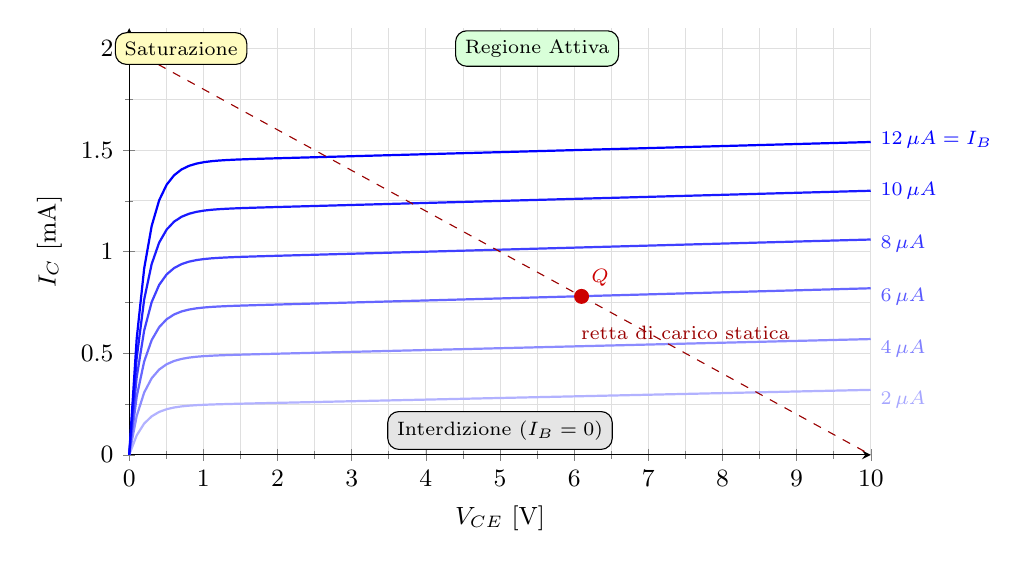
\begin{tikzpicture}
        \begin{axis}[
            xlabel={$V_{CE}$ [V]},
            ylabel={$I_C$ [mA]},
            xmin=0, xmax=10,
            ymin=0, ymax=2.1,
            axis lines=left,
            grid=both,
            grid style={line width=0.3pt, draw=gray!25},
            minor tick num=1,
            width=11cm, height=7cm,
            tick label style={font=\small},
            label style={font=\small},
            enlargelimits=false,
            clip=false,
        ]
        % Curve I_B = 2,4,6,8,10,12 uA
        \addplot[thick, blue!30,  domain=0:10, samples=100] {0.24*(1-exp(-5*x))+x*0.008};
        \addplot[thick, blue!45,  domain=0:10, samples=100] {0.48*(1-exp(-5*x))+x*0.009};
        \addplot[thick, blue!60,  domain=0:10, samples=100] {0.72*(1-exp(-5*x))+x*0.010};
        \addplot[thick, blue!75,  domain=0:10, samples=100] {0.96*(1-exp(-5*x))+x*0.010};
        \addplot[thick, blue!90,  domain=0:10, samples=100] {1.20*(1-exp(-5*x))+x*0.010};
        \addplot[thick, blue!100, domain=0:10, samples=100] {1.44*(1-exp(-5*x))+x*0.010};
        % Etichette curve
        \node[right, font=\scriptsize, blue!35]  at (axis cs:10, 0.27)  {$2\,\mu A$};
        \node[right, font=\scriptsize, blue!50]  at (axis cs:10, 0.52)  {$4\,\mu A$};
        \node[right, font=\scriptsize, blue!65]  at (axis cs:10, 0.78)  {$6\,\mu A$};
        \node[right, font=\scriptsize, blue!80]  at (axis cs:10, 1.04)  {$8\,\mu A$};
        \node[right, font=\scriptsize, blue!95]  at (axis cs:10, 1.30)  {$10\,\mu A$};
        \node[right, font=\scriptsize, blue!100] at (axis cs:10, 1.55)  {$12\,\mu A = I_B$};
        % Punto Q 
        \addplot[mark=*, mark size=2.5pt, red!80!black] coordinates {(6.1, 0.78)};
        \node[above right, font=\scriptsize, red!80!black] at (axis cs:6.1,0.78) {$Q$};
        % Retta di carico
        \addplot[dashed, red!60!black, domain=0:10, samples=2] {(10-x)/5.0};
        \node[font=\scriptsize, red!60!black] at (axis cs:7.5,0.6) {retta di carico statica};
        % Aree zones
        \node[draw, rounded corners, fill=yellow!25, font=\scriptsize]
             at (axis cs:0.7, 2.0) {Saturazione};
        \node[draw, rounded corners, fill=green!15, font=\scriptsize]
             at (axis cs:5.5, 2.0) {Regione Attiva};
        \node[draw, rounded corners, fill=gray!20, font=\scriptsize]
             at (axis cs:5.0, 0.12) {Interdizione ($I_B=0$)};
        \end{axis}
    \end{tikzpicture}
    \caption{Caratteristiche d'uscita $I_C(V_{CE})$ del modello CE ($\beta_F=120$). Si distinguono chiaramente le tre zone operative: saturazione, attiva e interdizione. La pendenza finita in regione attiva è indice dell'Effetto Early.}
\end{figure}

I parametri $H$ a piccolo segnale (modello ibrido) nel punto di riposo sono così definiti:
\begin{center}
\begin{adjustbox}{max width=\textwidth}
\renewcommand{\arraystretch}{1.3}
\begin{tabular}{cllll}
    \hline
    \textbf{Param.} & \textbf{Definizione Analitica} & \textbf{Espressione} & \textbf{Valore Tipico} & \textbf{Significato Fisico} \\
    \hline
    $h_{11}$ & $\partial v_{BE}/\partial i_B|_{v_{CE}=0}$ & $r_{BE} = mV_T/I_{BQ}$ & $\sim\!1\,\mathrm{k\Omega}$ & Resistenza dinamica ingresso \\
    $h_{21}$ & $\partial i_C/\partial i_B|_{v_{CE}=0}$   & $\beta_F$              & $50$--$500$               & Guadagno di corrente \\
    $h_{22}$ & $\partial i_C/\partial v_{CE}|_{i_B=0}$   & $1/r_{CE} \simeq 0$    & $\sim\!10^{-5}\,\mathrm{S}$ & Ammettanza d'uscita (Effetto Early) \\
    $h_{12}$ & $\partial v_{BE}/\partial v_{CE}|_{i_B=0}$ & $\simeq 0$            & $\ll 1$                   & Retroazione interna tensione \\
    \hline
\end{tabular}
\end{adjustbox}
\end{center}

\vspace{0.3cm}
\begin{definizione}{Effetto Early (Modulazione della Base)}
    All'aumentare della tensione $V_{CE}$, la regione di svuotamento della giunzione B--C (polarizzata inversamente) si espande. Questo fenomeno riduce la larghezza effettiva della base neutra ($W_B$), che è minore della larghezza metallurgica. 
    Di conseguenza, aumenta la probabilità che gli elettroni iniettati raggiungano il collettore (ovvero $\alpha_F \to 1$), producendo una lieve crescita lineare della corrente $I_C$ anche in regione attiva (rappresentata da $h_{22} \neq 0$). 
    Geometricamente, le curve caratteristiche prolungate all'indietro convergono in un punto sull'asse negativo delle tensioni pari a $-V_A$, definita \emph{Tensione di Early} ($V_A \approx 50$--$200\,\mathrm{V}$).
\end{definizione}

\begin{definizione}{Effetto Transistor}
    L'Effetto Transistor consiste nella capacità del dispositivo di trasferire una corrente da un circuito a bassa resistenza (giunzione B--E polarizzata direttamente) a uno ad altissima resistenza (giunzione B--C polarizzata inversamente); da qui il nome \emph{transistor}, contrazione di \emph{transfer resistor}.
    La gran parte dei portatori minoritari iniettati nella base la attraversa senza ricombinarsi e viene "catturata" dal forte campo elettrico della giunzione B--C, fluendo nel terminale di collettore.
\end{definizione}

\vspace{0.3cm}
\begin{osservazione}{Zone di Funzionamento Statiche}
    La barriera di potenziale $V_\gamma$ (knee voltage) dipende dal materiale semiconduttore impiegato: $V_\gamma \approx 0.6\,\mathrm{V}$ per il Silicio (Si) e $V_\gamma \approx 0.2\,\mathrm{V}$ per il Germanio (Ge). A seconda dello stato di polarizzazione delle giunzioni (Diretta = PD, Inversa = PI), il BJT opera in tre possibili regioni:

    \begin{center}
    \begin{adjustbox}{max width=\textwidth}
    \renewcommand{\arraystretch}{1.2}
    \begin{tabular}{llll}
        \hline
        \textbf{Zona} & \textbf{Giunzioni BE / BC} & \textbf{Condizione Tensione} & \textbf{Comportamento Circuitale} \\
        \hline
        \textbf{Attiva}      & PD / PI & $V_\gamma \lesssim V_{BE} < V_{CE}$ & Amplificazione ($I_C = \beta_F I_B$) \\
        \textbf{Saturazione} & PD / PD & $0 \lesssim V_{CE} < V_\gamma \lesssim V_{BE}$ & Interruttore \emph{ON} ($V_{CE,sat} \approx 0.2\,\mathrm{V}$) \\
        \textbf{Interdizione} & PI / PI & $V_{BE} < V_\gamma$ (es. $V_{BE} \le 0$) & Interruttore \emph{OFF} ($I_C \simeq 0$) \\
        \hline
    \end{tabular}
    \end{adjustbox}
    \end{center}
\end{osservazione}


% ============================================================
%  RIEPILOGO MODELLI EQUIVALENTI DEGLI AMPLIFICATORI
% ============================================================
% ============================================================
%  BREVE RECAP DEGLI AMPLIFICATORI
% ============================================================
\section{Breve Recap degli Amplificatori}
Qualsiasi amplificatore, se analizzato nel regime di piccolo segnale, può essere rappresentato come un quadripolo lineare. A seconda della natura della grandezza d'ingresso (Tensione o Corrente) e di quella d'uscita, risulta matematicamente più conveniente adottare uno dei tre modelli circuitali equivalenti.

\subsubsection*{1. Modello Equivalente di Thévenin (Tensione--Tensione)}
Il quadripolo viene sintetizzato mediante un'impedenza d'ingresso $Z_{in}$ posta ai terminali della porta entrante, seguita da una maglia d'uscita composta da un generatore di tensione controllato ($A_v v_{in}$) in serie a un'impedenza d'uscita $Z_{out}$.

    \begin{figure}[H]
        \centering
        \begin{circuitikz}[american, scale=0.95, transform shape]
            % Quadripolo Box
            \draw[thick, fill=noteblue!3, draw=noteblue!60!black, rounded corners=3pt] (1.8,-0.3) rectangle (8.2,2.3);
            
            % Ingresso
            \draw (0,2) to[short, i=$i_{in}$, o-] (1.8,2);
            \draw (0,0) to[short, o-] (1.8,0);
            \draw[<->, >=stealth] (0.3,1.8) -- (0.3,0.2) node[midway, fill=white, inner sep=1pt] {$v_{in}$};
            
            % Zin all'interno
            \draw (2.8,2) to[R, l=$Z_{in}$] (2.8,0);
            \draw (1.8,2) -- (2.8,2);
            \draw (1.8,0) -- (2.8,0);
            
            % Generatore controllato Av*vin e Zout in serie
            \draw (5.3,0) to[cV, l_=$A_v v_{in}$] (5.3,2) to[R, l=$Z_{out}$] (7.8,2);
            \draw (5.3,0) -- (7.8,0);
            
            % Uscita e Carico RL
            \draw (7.8,2) to[short, -o] (9.0,2);
            \draw (7.8,0) to[short, -o] (9.0,0);
            \draw[<->, >=stealth] (8.7,1.8) -- (8.7,0.2) node[midway, fill=white, inner sep=1pt] {$v_{out}$};
            
            \draw (9.0,2) to[short] (10.0,2) to[R, l=$R_L$] (10.0,0) to[short] (9.0,0);
        \end{circuitikz}
    \end{figure}

    Le relazioni circuitali salienti sono le seguenti:
    
    \textbf{Impedenza di Ingresso:} $Z_{in} = \frac{v_{in}}{i_{in}}$
    
    \textbf{Funzionamento a vuoto ($R_L \to \infty$):} $v_{out} = A_v\,v_{in}$
    
    \textbf{Funzionamento sotto carico ($R_L < \infty$):} A causa del partitore di tensione in uscita, il guadagno effettivo decresce:
        \[
            A'_v = \frac{v_{out}}{v_{in}} = A_v \left( \frac{R_L}{R_L + Z_{out}} \right)
        \]
        Per minimizzare questa perdita, un amplificatore di tensione ideale deve avere $Z_{out} \to 0$.

\subsubsection*{2. Modello Equivalente di Norton (Corrente--Corrente)}
    Rappresenta l'amplificatore modellando la porta di uscita come un generatore di corrente controllato ($A_i i_{in}$) posto in parallelo alla propria ammettanza d'uscita $1/Z_{out}$.

    \begin{figure}[H]
        \centering
        \begin{circuitikz}[american, scale=0.95, transform shape]
            % Quadripolo Box
            \draw[thick, fill=noteblue!3, draw=noteblue!60!black, rounded corners=3pt] (1.8,-0.3) rectangle (8.2,2.3);
            
            % Ingresso
            \draw (0,2) to[short, i=$i_{in}$, o-] (1.8,2);
            \draw (0,0) to[short, o-] (1.8,0);
            \draw[<->, >=stealth] (0.3,1.8) -- (0.3,0.2) node[midway, fill=white, inner sep=1pt] {$v_{in}$};
            
            % Zin
            \draw (2.8,2) to[R, l=$Z_{in}$] (2.8,0);
            \draw (1.8,2) -- (2.8,2);
            \draw (1.8,0) -- (2.8,0);
            
            % cI (generatore corrente controllato) e Zout in parallelo
            \draw (5.2,2) to[cI, l_=$A_i i_{in}$] (5.2,0);
            \draw (5.2,2) -- (7.2,2) to[R, l=$Z_{out}$, *-*] (7.2,0);
            \draw (7.2,2) -- (7.8,2);
            \draw (5.2,0) -- (7.8,0);
            
            % Uscita e Carico RL
            \draw (7.8,2) to[short, i=$i_{out}$, -o] (9.0,2);
            \draw (7.8,0) to[short, -o] (9.0,0);
            
            \draw (9.0,2) to[short] (10.0,2) to[R, l=$R_L$] (10.0,0) to[short] (9.0,0);
        \end{circuitikz}
    \end{figure}

    Le relazioni sono analoghe al duale di Thévenin, calcolate mediante partitore di corrente:
    
    \textbf{Funzionamento in corto circuito ($R_L = 0$):} $i_{out} = A_i\,i_{in}$
    
    \textbf{Funzionamento sotto carico ($R_L > 0$):}
        \[
            A'_i = \frac{i_{out}}{i_{in}} = A_i \left( \frac{Z_{out}}{Z_{out} + R_L} \right)
        \]
        Per un amplificatore di corrente ideale si desidera dunque $Z_{out} \to \infty$.

\subsubsection*{3. Modello a Parametri Ibridi (Parametri $H$)}
    La rappresentazione più naturale per il BJT è il modello a parametri ibridi, in cui la maglia di ingresso si comporta come un equivalente di Thévenin (serie), mentre la maglia di uscita come un equivalente di Norton (parallelo).

    \begin{figure}[H]
        \centering
        \begin{circuitikz}[american, scale=0.95, transform shape]
            % Quadripolo Box
            \draw[thick, fill=noteblue!3, draw=noteblue!60!black, rounded corners=3pt] (1.4,-0.3) rectangle (8.6,2.3);
            
            % Ingresso
            \draw (0,2) to[short, i=$i_{in}$, o-] (1.4,2);
            \draw (0,0) to[short, o-] (1.4,0);
            
            % h11 e h12*vout in serie
            \draw (1.4,2) to[R, l=$h_{11}$] (3.6,2) to[cV, l_=$h_{12} v_{out}$] (3.6,0) -- (1.4,0);
            
            % h21*i1 e h22 in parallelo
            \draw (5.8,0) -- (8.6,0);
            \draw (5.8,2) to[cI, l_=$h_{21} i_{in}$] (5.8,0);
            \draw (5.8,2) -- (7.6,2) to[R, l=$h_{22}^{-1}$, *-*] (7.6,0);
            \draw (7.6,2) -- (8.6,2);
            
            % Uscita e Carico RL
            \draw (8.6,2) to[short, i=$i_{out}$, -o] (9.6,2);
            \draw (8.6,0) to[short, -o] (9.6,0);
            
            \draw (9.6,2) to[short] (10.6,2) to[R, l=$R_L$] (10.6,0) to[short] (9.6,0);
        \end{circuitikz}
    \end{figure}

    Le equazioni costitutive in termini matriciali sono date da:
    \begin{equation}
        \begin{pmatrix} v_{in} \\ i_{out} \end{pmatrix} =
        \begin{pmatrix} h_{11} & h_{12} \\ h_{21} & h_{22} \end{pmatrix}
        \begin{pmatrix} i_{in} \\ v_{out} \end{pmatrix}
    \end{equation}
    ove, nel caso del BJT, $h_{11}=r_{BE}$, $h_{12}\simeq 0$, $h_{21}=\beta_F$, e $h_{22}=r_{CE}^{-1}$.

% ============================================================
%  AMPLIFICATORE CE CON RESISTENZA DI EMETTITORE
% ============================================================
\newpage
\section{Amplificatore di Tensione ad Emettitore Comune a Piccolo Segnale}

\subsection{Guadagno senza degenerazione d'emettitore}

\begin{teorema}{Guadagno dell'Amplificatore CE (Senza $R_E$)}
    Nel circuito a piccolo segnale a emettitore comune privo di resistenza di degenerazione ($R_E$), il transistor è fedelmente descritto mediante il suo modello ibrido-$\pi$.
    
    \begin{figure}[H]
        \centering
        \begin{circuitikz}[american, scale=0.9, transform shape]
            % Riquadro filtro
            \draw[thick, draw=red, rounded corners=4pt] (0.1, -0.6) rectangle (4.1, 2.9);
            \draw[thick, red, -stealth] (1.0, -0.6) |- (1.5, -1.0);
            \node[font=\normalsize\itshape, text=black, anchor=west] at (1.5, -1.0) {filtro passa alto necessario per bloccare le frequenze di fondo};
            
            % Sorgente Vs
            \draw (0,2) to[short, o-] (0.5,2);
            \draw (0,0) to[short, o-] (0.5,0);
            \node at (-0.4, 1) {$v_s$};
            
            % Filtro Passa Alto (C, R2, R1)
            \draw (0.5,2) to[C, l=$C$] (2,2);
            \draw (0.5,0) -- (2,0);
            \draw (2,2) to[R, l=$R_2$, *-*] (2,0);
            \draw (2,2) -- (3.5,2);
            \draw (2,0) -- (3.5,0);
            \draw (3.5,2) to[R, l=$R_1$, *-*] (3.5,0);
            \draw (2.75,0) node[ground]{}; % Messa a terra
            
            % Connessioni a Base e E
            \draw (3.5,2) -- (4.2,2);
            \draw (3.5,0) -- (4.2,0);
            
            % Terminali allineati
            \draw (4.2,2) -- (5.0,2);
            \node[ocirc] at (4.6, 2) {};
            \node[above, font=\large] at (4.6, 2.1) {B};
            
            \draw (4.2,0) -- (5.0,0);
            \node[ocirc] at (4.6, 0) {};
            \node[below, font=\large] at (4.6, -0.1) {E};
            
            % Corrente i_B
            \draw[->, thick, black] (4.3, 2.4) -- (4.9, 2.4) node[midway, above, font=\large] {$i_b$};
            
            % BJT Box
            \draw[thick, draw=gray, rounded corners=2pt] (5.3, -0.4) rectangle (9.7, 2.6);
            
            % Modello BJT (ibrido-pi)
            \draw (5.0,2) -- (5.8,2) to[R, l=$r_{BE}$] (7.2,2) -- (7.2,0);
            \draw (8.8,2) to[cI, l_=$\beta_F i_b$] (8.8,0);
            \draw (8.8,2) -- (10.0,2);
            
            % Linea Emettitore continua
            \draw (5.0,0) -- (10.0,0);
            
            % Nodo C e E in uscita
            \node[ocirc] at (10.6, 2) {};
            \node[above, font=\large] at (10.6, 2.1) {C};
            \node[ocirc] at (10.6, 0) {};
            \node[below, font=\large] at (10.6, -0.1) {E};
            
            % Corrente i_C
            \draw[<-, thick, black] (10.3, 2.4) -- (10.9, 2.4) node[midway, above, font=\large] {$i_c$};
            
            % Rc e Uscita
            \draw (10.0,2) -- (11.5,2) to[R, l=$R_C$, *-*] (11.5,0) -- (10.0,0);
            \draw (11.5,2) to[short, -o] (12.5,2);
            \draw (11.5,0) to[short, -o] (12.5,0);
        \end{circuitikz}
        \caption{Circuito equivalente a piccolo segnale per l'amplificatore CE senza $R_E$.}
    \end{figure}

    Dall'analisi delle maglie, sapendo che $v_{be} = r_{BE} i_b$ e $v_{out} = -R_C i_c = -R_C \beta_F i_b$, il guadagno di tensione $A_V$ (tra il collettore e la base) risulta:
    \begin{equation}
        A_V = \frac{v_{out}}{v_{be}} = -\frac{\beta_F R_C}{r_{BE}}
    \end{equation}
    Tale guadagno è intrinsecamente elevato ($|A_V| \ge 100$), tuttavia soffre di una \textbf{forte indeterminazione}, in quanto il parametro $r_{BE} = mV_T / I_{BQ}$ e il beta $\beta_F$ dipendono marcatamente dal punto di lavoro in continua e dalle variazioni termiche, minando la stabilità progettuale del circuito.
\end{teorema}

\subsection{Guadagno con resistenza di degenerazione $R_E$}

\begin{teorema}{Guadagno dell'Amplificatore CE (Con $R_E$)}
    Per svincolare il guadagno di tensione dalla dipendenza dai parametri intrinseci fluttuanti del transistor, si inserisce una resistenza di degenerazione $R_E$ sul ramo dell'emettitore.
    
    \begin{figure}[H]
        \centering
        \begin{circuitikz}[american, scale=0.9, transform shape]
            % Sorgente Vs
            \draw (0,2) to[short, o-] (0.5,2);
            \draw (0,0) to[short, o-] (0.5,0);
            \node at (-0.4, 1) {$v_s$};
            
            % Filtro Passa Alto (C, R2, R1)
            \draw (0.5,2) to[C, l=$C$] (2,2);
            \draw (0.5,0) -- (2,0);
            \draw (2,2) to[R, l=$R_2$, *-*] (2,0);
            \draw (2,2) -- (3.5,2);
            \draw (2,0) -- (3.5,0);
            \draw (3.5,2) to[R, l=$R_1$, *-*] (3.5,0);
            \draw (2.75,0) node[ground]{}; % Messa a terra
            
            % Connessioni a Base
            \draw (3.5,2) -- (4.2,2);
            \draw (3.5,0) -- (4.2,0);
            
            \draw (4.2,2) -- (5.0,2);
            \node[ocirc] at (4.6, 2) {};
            \node[above, font=\large] at (4.6, 2.1) {B};
            
            \draw (4.2,0) -- (5.0,0);
            \node[ocirc] at (4.6, 0) {};
            \node[below, font=\large] at (4.6, -0.1) {E};
            
            % Corrente i_B
            \draw[->, thick, black] (4.3, 2.4) -- (4.9, 2.4) node[midway, above, font=\large] {$i_b$};
            
            % Corrente i_E in basso
            \draw[->, thick, black] (5.2, -0.5) -- (5.8, -0.5) node[midway, below, font=\large] {$i_e$};
            
            % R_E orizzontale
            \draw[thick, draw=red, rounded corners=2pt] (5.2, -0.4) rectangle (6.8, 0.4);
            \draw (5.0,0) to[R, l=$R_E$] (7.0,0);
            
            % BJT Box
            \draw[thick, draw=gray, rounded corners=2pt] 
                (5.5, 2.6) -- (10.2, 2.6) -- (10.2, -0.4) -- (7.3, -0.4) -- (7.3, 0.6) -- (5.5, 0.6) -- cycle;
                
            % Modello BJT
            \draw (5.0,2) -- (6.3,2) to[R, l=$r_{BE}$] (7.7,2) -- (7.7,0);
            \draw (9.3,2) to[cI, l_=$\beta_F i_b$] (9.3,0);
            \draw (9.3,2) -- (10.5,2);
            
            \draw (7.0,0) -- (10.5,0);
            
            % Nodi C ed E
            \node[ocirc] at (11.1, 2) {};
            \node[above, font=\large] at (11.1, 2.1) {C};
            \node[ocirc] at (11.1, 0) {};
            \node[below, font=\large] at (11.1, -0.1) {E};
            
            % Corrente i_C
            \draw[<-, thick, black] (10.8, 2.4) -- (11.4, 2.4) node[midway, above, font=\large] {$i_c$};
            
            % Rc e Uscita
            \draw[gray] (10.5,2) -- (12.0,2) to[R, l=$R_C$, color=gray, *-*] (12.0,0) -- (10.5,0);
            \draw[gray] (12.0,2) to[short, -o] (13.0,2);
            \draw[gray] (12.0,0) to[short, -o] (13.0,0);
        \end{circuitikz}
        \caption{Circuito equivalente a piccolo segnale per l'amplificatore CE stabilizzato con $R_E$.}
    \end{figure}

    Risolvendo la maglia di ingresso a valle del partitore resistivo (base--$r_{BE}$--$R_E$--massa), la tensione sulla base è data da:
    \begin{equation*}
        v_b = r_{BE} i_b + R_E i_e = \left[ r_{BE} + (1+\beta_F)R_E \right] i_b \qquad \text{essendo } i_e = (1+\beta_F)i_b
    \end{equation*}
    Da cui si evince una fondamentale conseguenza: l'impedenza di ingresso alla base risulta notevolmente innalzata dall'effetto di $R_E$:
    \begin{equation}
        Z_{in,base} = \frac{v_b}{i_b} = r_{BE} + (1+\beta_F)R_E \gg r_{BE}
    \end{equation}
    Il segnale in uscita sul collettore vale $v_{out} = v_c = -R_C i_c = -R_C \beta_F i_b$. Il guadagno di tensione complessivo (dalla base al collettore) assume dunque la forma:
    \begin{equation}
        A_V = \frac{v_{out}}{v_b} = -\frac{\beta_F R_C}{r_{BE} + (1+\beta_F)R_E}
    \end{equation}
    Nel limite pratico in cui il termine di degenerazione domina ($R_E \gg r_{BE}/\beta_F$), la formula si approssima a:
    \begin{equation}
        A_V \simeq -\frac{R_C}{R_E}
    \end{equation}
    Questa approssimazione assicura che il guadagno sia fissato unicamente dal rapporto tra componenti passivi esterni, rendendo il circuito estremamente stabile e robusto rispetto alle tolleranze di $\beta_F$.

    \vspace{0.2cm}
    Tuttavia, permane un problema di conflitto: un elevato $|A_V|$ impone di scegliere una $R_C$ molto grande. Essendo l'impedenza di uscita del circuito proprio $Z_{out} \simeq R_C$, il segnale verrà fortemente attenuato qualora l'amplificatore dovesse pilotare carichi a bassa impedenza. La soluzione tipica a questo conflitto è l'inserimento in cascata di un \emph{buffer} (ad esempio uno stadio a Collettore Comune) che disaccoppi le impedenze.
\end{teorema}

% ============================================================
%  CC E RETE DI POLARIZZAZIONE
% ============================================================
\subsection{Configurazione a collettore comune (buffer)}

\begin{osservazione}{Configurazione a Collettore Comune (Inseguitore o Buffer)}
    Lo stadio a collettore comune viene tipicamente posto a cascata dopo l'amplificatore di tensione per effettuare l'adattamento di impedenza. Risolvendo le equazioni ai piccoli segnali per questa topologia, si evincono le seguenti proprietà chiave:
    \begin{itemize}[label=$\cdot$, leftmargin=*]
        \item \textbf{Guadagno di Tensione Unitario:} $A_v \simeq 1$. Il potenziale dell'emettitore "insegue" (\emph{follower}) fedelmente quello della base.
        \item \textbf{Alta Impedenza di Ingresso:} $Z_{in} = r_{BE} + (1+\beta_F)R_E$, in virtù della degenerazione indotta dal carico sull'emettitore (stessa formula dell'amplificatore CE con $R_E$).
        \item \textbf{Bassa Impedenza di Uscita:} $Z_{out} \simeq \frac{r_{BE} + R_S}{1+\beta_F} \sim 10\,\Omega$ (con $R_S$ resistenza della sorgente). Questa proprietà lo rende un traslatore d'impedenza formidabile, ideale per pilotare carichi senza attenuare il segnale.
    \end{itemize}
\end{osservazione}

\vspace{0.3cm}
\subsection{Rete di polarizzazione e punto di riposo}

\begin{esercizio}{Rete di Polarizzazione (Punto di Quiescenza)}
    Al fine di garantire il corretto funzionamento del transistor nel regime lineare (zona attiva), è imperativo stabilirne in modo univoco il \textbf{punto di lavoro in DC (quiescenza)}. La tecnica standard sfrutta un partitore resistivo sulla base, semplificabile mediante l'applicazione del \textbf{Teorema di Thévenin} (\Cref{sec:thevenin}).

    \vspace{0.3cm}
    \begin{center}
        \begin{minipage}[c]{0.45\textwidth}
            \centering
            \begin{circuitikz}[american, scale=0.85, transform shape]
                \draw (0,0) node[npn](Q){};
                \draw (Q.B) -- ++(-1.5,0) coordinate(B);
                \draw (B) to[R, l_=$R_1$] ++(0,2.5) node[above]{$V_{CC}$};
                \draw (B) to[R, l=$R_2$] ++(0,-2.5) node[ground]{};
                \draw (Q.C) to[R, l_=$R_C$] ++(0,2.5) node[above]{$V_{CC}$};
                \draw (Q.E) to[R, l=$R_E$] ++(0,-2.5) node[ground]{};
            \end{circuitikz}
        \end{minipage}%
        \begin{minipage}[c]{0.1\textwidth}
            \centering
            $\xrightarrow{\text{Thévenin}}$
        \end{minipage}%
        \begin{minipage}[c]{0.45\textwidth}
            \centering
            \begin{circuitikz}[american, scale=0.85, transform shape]
                \draw (0,0) node[npn](Q){};
                \draw (Q.B) to[R, l_=$R_{BB}$] ++(-2,0) coordinate(VBB_top);
                \draw (VBB_top) to[vsource, l_=$V_{BB}$] ++(0,-2.5) node[ground]{};
                \draw (Q.C) to[R, l_=$R_C$] ++(0,2.5) node[above]{$V_{CC}$};
                \draw (Q.E) to[R, l=$R_E$] ++(0,-2.5) node[ground]{};
            \end{circuitikz}
        \end{minipage}
    \end{center}
    
    Il generatore equivalente $V_{BB}$ e l'impedenza equivalente $R_{BB}$ valgono:
    \begin{equation}
        V_{BB} = V_{CC} \frac{R_2}{R_1+R_2} \qquad \qquad R_{BB} = R_1 \parallel R_2
    \end{equation}

    \vspace{0.4cm}
    \textbf{Analisi Topologica delle Maglie} \\
    Sostituiamo il circuito originale con l'equivalente alla porta di base ed evidenziamo le due maglie principali.
    
    \vspace{0.2cm}
    \begin{center}
        \begin{circuitikz}[american, scale=1.0, transform shape]
            \draw (0,0) node[npn](Q){};
            
            \coordinate (GND) at (0,-3.5);
            
            % Maglia di ingresso
            \draw (Q.B) to[R, l_=$R_{BB}$] ++(-2.5,0) coordinate(VBB_top);
            \draw (VBB_top) to[vsource, l_=$V_{BB}$] (VBB_top |- GND) node[ground]{};
            
            % Maglia di uscita
            \draw (Q.E) to[R, l=$R_E$] (Q.E |- GND) node[ground]{};
            \draw (Q.C) to[R, l_=$R_C$] ++(0,2.5) coordinate(VCC_top) -- ++(3,0) coordinate(VCC_right);
            \draw (VCC_right) to[battery1, l=$V_{CC}$] (VCC_right |- GND) node[ground]{};
            
            % Evidenziatori rossi (Maglia IN e OUT)
            \draw[red, thick, rounded corners=8pt, dashed] (-4.3, -3.8) rectangle (-0.4, 0.8);
            \node[red, font=\bfseries] at (-2.3, 1.2) {Maglia IN};
            
            \draw[red, thick, rounded corners=8pt, dashed] (-0.3, -3.5) rectangle (0.5, 3.2);
            \node[red, font=\bfseries] at (0.45, 3.6) {Maglia OUT};
            
            % Correnti direzionali
            \draw[->, red, thick] (-2.2, -0.6) -- (-1.2, -0.6) node[midway, below]{$I_B$};
            \draw[->, red, thick] (1.1, 2.2) -- (1.1, 1.2) node[midway, right]{$I_C$};
            \draw[->, red, thick] (1.1, -1.2) -- (1.1, -2.2) node[midway, right]{$I_E$};
        \end{circuitikz}
    \end{center}
    
    \vspace{0.4cm}
    \textbf{1. Soluzione della Maglia di Ingresso (Circuito Base-Emettitore)} \\
    Applicando la Legge di Kirchhoff delle Tensioni (LKT) alla maglia di ingresso, formata dal generatore $V_{BB}$, $R_{BB}$, giunzione base-emettitore e $R_E$:
    \begin{equation}
        V_{BB} - R_{BB} I_B - V_{BE} - R_E I_E = 0
    \end{equation}
    Ponendo $I_E = (1+\beta_F)I_B$ e assumendo la giunzione polarizzata direttamente ($V_{BE} \simeq V_\gamma$), si ottiene il calcolo diretto per la corrente di base:
    \begin{equation}
        I_{BQ} = \frac{V_{BB} - V_\gamma}{R_{BB} + (1+\beta_F)R_E}
    \end{equation}
    La corrente di collettore nel punto di lavoro discende proporzionalmente $I_{CQ} = \beta_F I_{BQ}$. Si nota che, in buona progettazione (se $\beta_F R_E \gg R_{BB}$), la corrente si stabilizza al valore $I_{CQ} \approx (V_{BB} - V_\gamma)/R_E$, indipendente dal parametro dispersivo $\beta_F$.

    \vspace{0.4cm}
    \textbf{2. Soluzione della Maglia di Uscita (Circuito Collettore-Emettitore)} \\
    Per chiudere il problema e localizzare precisamente il punto sulle caratteristiche, scriviamo la LKT lungo la maglia di uscita:
    \begin{equation}
        V_{CC} = R_C I_{CQ} + V_{CEQ} + R_E I_{EQ}
    \end{equation}
    Approssimando $I_{EQ} \simeq I_{CQ}$, poiché $\alpha_F \approx 1$, determiniamo la caduta di tensione ai morsetti di uscita in conduzione quieta:
    \begin{equation}
        V_{CEQ} = V_{CC} - (R_C+R_E)I_{CQ}
    \end{equation}
\end{esercizio}

\vspace{0.3cm}
\noindent \textbf{Condizione di validità (ZAD):} \\
Affinché il transistor operi correttamente in \textbf{Zona Attiva Diretta (ZAD)}, che è la condizione necessaria per l'amplificazione lineare, la giunzione collettore-base deve rimanere polarizzata inversamente. Questo si traduce nella disuguaglianza operativa:
\begin{equation}
    V_{CEQ} > V_{BEQ} \simeq V_\gamma > 0
\end{equation}

\subsection{Comportamento alle alte frequenze ed effetto Miller}
\label{sec:miller-bjt}

\begin{osservazione}{Comportamento del BJT ad Alta Frequenza}
    Il modello a piccolo segnale a bassa frequenza non è sufficiente per descrivere il comportamento del BJT quando il segnale d'ingresso ha variazioni rapide. Ad alte frequenze, subentrano gli effetti delle \textbf{capacità parassite} intrinseche delle giunzioni a semiconduttore, in particolare la capacità base-emettitore ($C_{BE}$) e la capacità base-collettore ($C_{BC}$).
    
    \vspace{0.2cm}
    \begin{center}
        \begin{circuitikz}[american, scale=1.3, transform shape]
            % Base
            \draw (0,0) node[ocirc]{} node[left, font=\large]{B} -- (1,0) coordinate(b_node);
            % Collector
            \draw (b_node) to[C, l=$C_{BC}$] (3.5,0) coordinate(c_node) -- (4.5,0) node[ocirc]{} node[above, font=\large]{C};
            
            % Emitter line (bottom)
            \draw (0,-2.5) node[ocirc]{} node[left, font=\large]{E} -- (4.5,-2.5) node[ocirc]{} node[below, font=\large]{E};
            
            % C_BE and r_BE in parallel
            \draw (b_node) -- (1,-0.5) coordinate(split_b);
            \draw (split_b) -- (0.2,-0.5) to[C, l_=$C_{BE}$] (0.2,-2) -- (0.2,-2.5);
            \draw (split_b) -- (1.8,-0.5) to[R, l=$r_{BE}$] (1.8,-2) -- (1.8,-2.5);
            
            % Dependent source
            \draw (c_node) to[cI, l=$\beta_F i_b$] (c_node |- 0,-2.5);
        \end{circuitikz}
    \end{center}
    
    \vspace{0.2cm}
    Il decadimento delle prestazioni ad alta frequenza si spiega come segue:
    \begin{itemize}[label=$\cdot$, leftmargin=*]
        \item Nel regime a \textbf{basse frequenze}, l'impedenza di questi condensatori ($Z_C = 1/j\omega C$) è asintoticamente elevata. Essi appaiono come circuiti aperti e non alterano il calcolo del guadagno.
        \item Nel regime ad \textbf{alte frequenze}, l'impedenza capacitiva crolla, offrendo percorsi a bassa reattanza. Una frazione crescente della corrente di segnale in ingresso si scarica a massa attraverso $C_{BE}$, bypassando la resistenza $r_{BE}$. Contemporaneamente, la capacità $C_{BC}$ introduce un percorso di retroazione negativa (feedback) dal nodo di collettore al nodo di base, abbattendo drasticamente il guadagno di tensione complessivo del dispositivo.
    \end{itemize}
\end{osservazione}

\vspace{0.3cm}
L'impatto della capacità di retroazione $C_{BC}$ sulle prestazioni del circuito è formalmente quantificato attraverso un celebre risultato dell'analisi delle reti elettriche: il \textbf{Teorema di Miller}.

\begin{teorema}{Effetto Miller e Prodotto Banda-Guadagno}
    Il Teorema di Miller stabilisce che un'impedenza trasversale $Z$, collegata tra due nodi la cui differenza di potenziale è vincolata dalla relazione lineare $v_2 = A v_1$ (dove $A$ è l'amplificazione invertente tra i due nodi), può essere sdoppiata in due impedenze equivalenti verso massa.
    
    \vspace{0.2cm}
    \begin{center}
        \begin{circuitikz}[american, scale=1.2, transform shape]
            % Box centrale
            \draw[thick] (1.5,-1) rectangle (3.5,1) node[midway]{\Large $A$};
            
            % Linee orizzontali
            \draw (0,0.5) to[short, o-] (1.5,0.5);
            \draw (0,-0.5) to[short, o-] (1.5,-0.5);
            \draw (3.5,0.5) to[short, -o] (5,0.5);
            \draw (3.5,-0.5) to[short, -o] (5,-0.5);
            
            % Tensioni
            \draw[<->] (0, 0.4) -- (0, -0.4) node[midway, left]{$v_1$};
            \draw[<->] (5, 0.4) -- (5, -0.4) node[midway, right]{$v_2$};
            
            % Z trasversale originaria
            \draw (0.8, 0.5) -- (0.8, 2.0) to[generic, l_=$Z$] (4.2, 2.0) -- (4.2, 0.5);
            \draw[->, gray, thick] (1.5, 2.6) -- (3.5, 2.6) node[midway, above]{$I_Z$};
            
            % Equivalent Z1, Z2
            \draw[thick, dashed] (0.8, 0.5) to[generic, l_=$Z_{in}$] (0.8, -0.5);
            \draw[thick, dashed] (4.2, 0.5) to[generic, l=$Z_{out}$] (4.2, -0.5);
        \end{circuitikz}
    \end{center}
    
    \vspace{0.2cm}
    La corrente che fluisce nell'impedenza $Z$ vale $I_Z = \frac{v_1 - v_2}{Z} = \frac{v_1(1-A)}{Z}$. Dal punto di vista del nodo di ingresso ($v_1$), il circuito assorbe la medesima corrente se $Z$ viene sostituita da un'impedenza equivalente verso massa pari a:
    \begin{equation}
        Z_{in} = \frac{Z}{1-A}
    \end{equation}
    Analogamente, per il nodo di uscita, l'impedenza equivalente verso massa risulta:
    \begin{equation}
        Z_{out} = \frac{Z}{1 - 1/A} = \frac{A}{A-1} Z
    \end{equation}
    
    Nel caso specifico di un amplificatore ad emettitore comune invertente ($A \ll -1$), la capacità $C_{BC}$ assume il ruolo di $Z$ ($Z = 1/j\omega C_{BC}$). Applicando la scomposizione di Miller, l'impedenza riportata in ingresso è una capacità equivalente $C_{M1}$:
    \begin{equation}
        C_{M1} = C_{BC}(1 - A) \simeq C_{BC}(1 + |A|)
    \end{equation}
    Questa equazione rivela che la capacità effettiva vista all'ingresso viene \textbf{moltiplicata} per il modulo del guadagno. Questo fenomeno, noto come Effetto Miller, causa un drastico calo dell'impedenza d'ingresso alle alte frequenze, determinando l'insorgere di un polo dominante che fissa la frequenza di taglio superiore ($f_H$) del sistema.
    
    L'Effetto Miller porta all'invarianza del \textbf{Prodotto Banda-Guadagno} (Gain-Bandwidth Product, GBWP): un tentativo di aumentare il guadagno di tensione $|A|$ provocherà un proporzionale incremento della capacità $C_{M1}$ e una conseguente riduzione della larghezza di banda dell'amplificatore, mantenendo approssimativamente costante il prodotto $A \cdot f_H$.
\end{teorema}


% ============================================================
%  TRANSISTOR DARLINGTON
% ============================================================
\subsection{Configurazione Darlington}

\begin{definizione}{Configurazione Darlington}
    La configurazione \emph{Darlington} è una topologia circuitale formata da due transistor bipolari collegati in cascata (direttamente accoppiati), in modo che la corrente di emettitore del primo piloti la corrente di base del secondo. L'intero blocco si comporta a tutti gli effetti come un singolo macro-transistor avente un guadagno di corrente straordinariamente elevato.
    
    \vspace{0.2cm}
    \begin{figure}[H]
        \centering
        \begin{circuitikz}[american, transform shape, scale=0.9]
            \draw (0,0) node[npn] (Q1) {1};
            \draw (1.5,-1) node[npn] (Q2) {2};
            \draw (Q1.E) -- (Q1.E |- Q2.B) -- (Q2.B);
            \draw (Q1.C) -- (0,1.5) -- (1.5,1.5) -- (Q2.C);
            \draw (1.5,1.5) -- (1.5,2) node[above] {$V_{CC}$};
            \draw (Q2.E) -- (1.5,-2) to[R, l=$R_E$] (1.5,-3) node[ground]{};
            \draw (Q1.B) -- (-1,0) node[ocirc]{} node[left, font=\large] {$v_s$};
            \draw (1.5,-2) to[short, *-o] (2.5,-2) node[right, font=\large] {$v_{out}$};
        \end{circuitikz}
        \caption{Coppia Darlington usata come stadio a collettore comune (emitter follower).}
    \end{figure}
    
    Analiticamente, supponendo per semplicità che i due transistor abbiano caratteristiche omogenee ($\beta_1 \approx \beta_2 = \beta_F \gg 1$), le correnti si legano come segue:
    \begin{align*}
        I_{C1} &= \beta_F i_{B1} \\
        i_{B2} &= i_{E1} = (1+\beta_F) i_{B1} \simeq \beta_F i_{B1} \\
        I_{C2} &= \beta_F i_{B2} \simeq \beta_F^2 i_{B1}
    \end{align*}
    La corrente di collettore totale del macro-dispositivo è dominata dal secondo stadio:
    \begin{equation}
        I_{C,TOT} = I_{C1} + I_{C2} \simeq \beta_F^2 i_{B1}
    \end{equation}
    Il sistema esibisce un guadagno di corrente equivalente $\beta_{eq} \simeq \beta_F^2$. Impiegato tipicamente come \emph{emitter follower}, il Darlington vanta:
    \begin{itemize}[label=$\cdot$, leftmargin=*]
        \item \textbf{Guadagno di tensione} asintotico a $1$ ($v_{out} \simeq v_s$).
        \item \textbf{Impedenza d'ingresso immensa} ($Z_{in} \propto \beta_F^2 R_E$).
        \item \textbf{Impedenza d'uscita infinitesima} ($Z_{out} \propto \beta_F^{-2}$).
    \end{itemize}
    
    Un inconveniente risiede nella polarizzazione in continua: se l'ingresso è accoppiato in DC, la tensione sul carico risulta traslata di due cadute di giunzione rispetto all'ingresso ($v_s \simeq v_{out} + 2V_\gamma$). Inoltre, aggiungere ulteriori transistor in cascata è poco pratico: il primo transistor lavorerebbe con correnti piccolissime (dove $\beta$ è più basso e le correnti di perdita diventano rilevanti) e le cadute $V_\gamma$ si sommerebbero.
\end{definizione}

% ============================================================
%  STADIO PUSH-PULL
% ============================================================
\subsection{Stadio push-pull (simmetria complementare)}

\begin{definizione}{Stadio a Simmetria Complementare (Push-Pull)}
    Per incrementare drasticamente l'efficienza degli amplificatori di potenza e consentire escursioni di segnale bipolari, si accoppiano due transistor a polarità opposta (un NPN e un PNP) in una topologia \emph{Push-Pull} simmetrica. 
    
    Il fondamento di questa architettura è che i due dispositivi lavorano in \textbf{alternanza}: in classe B non conducono mai contemporaneamente, ognuno amplifica una sola semionda. Non essendoci una rete di polarizzazione, a riposo nessuno dei due conduce (nessuna potenza dissipata) e l'ingresso è accoppiato direttamente, senza condensatori.
    
    \vspace{0.2cm}
    \begin{figure}[H]
        \centering
        \begin{circuitikz}[american, transform shape, scale=0.9]
            \draw (0,2) node[npn] (Q1) {NPN};
            \draw (0,-2) node[pnp] (Q2) {PNP};
            \draw (Q1.B) -- (Q2.B);
            \draw (Q1.B |- 0,0) to[short, *-o] (-1.5,0) node[left, font=\large] {$v_s$};
            \draw (Q1.E) -- (Q2.E);
            \draw (Q1.C) -- (0,3.5) node[above] {$+V_{CC}$};
            \draw (Q2.C) -- (0,-3.5) node[below] {$-V_{EE}$};
            \draw (Q1.E |- 0,0) to[short, *-] (1.5,0) to[R, l=$R_L$] (1.5,-2) node[ground]{};
            \draw (1.5,0) to[short, *-o] (2.5,0) node[right, font=\large] {$v_{out}$};
        \end{circuitikz}
        \caption{Stadio a simmetria complementare (Push-Pull in Classe B).}
    \end{figure}
    
    Il comportamento dell'amplificatore è dicotomico:
    \begin{itemize}[label=$\cdot$, leftmargin=*]
        \item \textbf{Semiciclo Positivo ($v_s > 0$):} Il transistor NPN si attiva fungendo da \emph{emitter follower}, mentre il PNP è interdetto. L'uscita insegue l'ingresso decurtato della soglia di giunzione: $v_{out} \simeq v_s - V_\gamma > 0$.
        \item \textbf{Semiciclo Negativo ($v_s < 0$):} L'NPN si spegne ed entra in conduzione il PNP, che assorbe la corrente dal carico verso $-V_{EE}$. La relazione diventa $v_{out} \simeq v_s + V_\gamma < 0$.
    \end{itemize}
    
    \vspace{0.3cm}
    \textbf{Distorsione di Cross-Over e Compensazione} \\
    Sussiste un intervallo critico in cui la tensione di segnale, pur non essendo nulla, è in modulo insufficiente a vincere la soglia di accensione delle giunzioni ($-V_\gamma < v_s < V_\gamma$). In questa regione detta \emph{banda morta}, ambo i dispositivi sono interdetti e $v_{out} = 0$. Ciò corrompe il segnale riprodotto generando la distorsione di \emph{cross-over}.
    
    \vspace{0.2cm}
    \begin{figure}[H]
        \centering
        \begin{circuitikz}[american, transform shape, scale=0.9]
            \draw (0,2) node[npn] (Q1) {};
            \draw (0,-2) node[pnp] (Q2) {};
            \draw (Q1.C) -- (0,3.5) node[above] {$+V_{CC}$};
            \draw (Q2.C) -- (0,-3.5) node[below] {$-V_{EE}$};
            \draw (Q1.E) -- (Q2.E);
            \draw (Q1.E |- 0,0) to[short, *-o] (2,0) node[right, font=\large] {$v_{out}$};
            \draw (Q1.B) -- (-2,2) to[D, l=$D_1$, *-*] (-2,0) to[D, l=$D_2$, -*] (-2,-2) -- (Q2.B);
            \draw (-2,2) to[R, l=$R_1$] (-2,3.5) node[above] {$+V_{CC}$};
            \draw (-2,-2) to[R, l=$R_2$] (-2,-3.5) node[below] {$-V_{EE}$};
            \draw (-2,0) to[short, -o] (-3.5,0) node[left, font=\large] {$v_s$};
        \end{circuitikz}
        \caption{Push-pull polarizzato in Classe AB mediante diodi traslatori.}
    \end{figure}
    
    La soluzione per abbattere il cross-over risiede nella topologia in \textbf{Classe AB}: l'inserimento di due diodi polarizzati direttamente (tramite $R_1$ e $R_2$) sul cammino del segnale trasla staticamente i potenziali di base dei transistor di quantità coincidenti alle tensioni di soglia ($V_{\gamma d} \approx V_\gamma$). In tale assetto, i dispositivi si trovano sull'imminenza della conduzione, cancellando l'intervallo morto di commutazione.
\end{definizione}

% ============================================================
%  AMPLIFICATORE DIFFERENZIALE
% ============================================================
\subsection{Amplificatore differenziale a BJT}

\begin{definizione}{Amplificatore Differenziale a BJT}
    L'amplificatore differenziale costituisce lo stadio d'ingresso d'elezione per quasi tutti i circuiti integrati moderni. La sua architettura genera un segnale d'uscita proporzionale esclusivamente alla \textbf{differenza tra due segnali di ingresso indipendenti}, eliminando i contributi comuni ai due ingressi.
    
    Si definiscono analiticamente due stimoli canonici:
    \begin{itemize}[label=$\cdot$, leftmargin=*]
        \item \textbf{Tensione di modo differenziale ($v_d$):} $v_d = v_1 - v_2$, che rappresenta l'informazione utile.
        \item \textbf{Tensione di modo comune ($v_c$):} $v_c = \frac{v_1 + v_2}{2}$, dovuta tipicamente a disturbi comuni ai due ingressi (rumore, interferenze, derive termiche).
    \end{itemize}
    In regime lineare, il potenziale in uscita si modella come combinazione lineare dei modi:
    \begin{equation}
        v_{out} = A_d v_d + A_c v_c
    \end{equation}
    Il pregio topologico si misura attraverso il \textbf{Rapporto di Reiezione di Modo Comune (CMRR)}:
    \begin{equation}
        \text{CMRR} = \left| \frac{A_d}{A_c} \right|
    \end{equation}
    Un differenziale ideale (CMRR asintotico a infinito) rigetta completamente le componenti concordi, amplificando unicamente la pura differenza.
    
    \vspace{0.3cm}
    La materializzazione in logica BJT avviene mediante una rete perfettamente simmetrica:
    \begin{figure}[H]
        \centering
        \begin{circuitikz}[american, transform shape, scale=0.9]
            \draw (-1.5,0) node[npn] (Q1) {};
            \draw (1.5,0) node[npn, xscale=-1] (Q2) {};
            
            % Resistori e Collettori
            \draw (Q1.C) to[R, l=$R_C$] (-1.5,2.5) -- (0,2.5) node[above, font=\large] {$+V_{CC}$} -- (1.5,2.5) to[R, l_=$R_C$] (Q2.C);
            
            % Emettitori accoppiati
            \draw (Q1.E) -- (-1.5,-1.2) -- (0,-1.2) -- (1.5,-1.2) -- (Q2.E);
            
            % Resistenza coda Emettitore
            \draw (0,-1.2) to[R, l=$R_E$] (0,-3.2) node[below, font=\large]{$-V_{EE}$};
            
            % Ingressi
            \draw (Q1.B) to[short, -o] (-2.5,0) node[left, font=\large] {$v_1$};
            \draw (Q2.B) to[short, -o] (2.5,0) node[right, font=\large] {$v_2$};
            
            % Uscite differenziali
            \draw (Q1.C) to[short, *-o] ++(-1,0) node[left, font=\large] {$v_{out1}$};
            \draw (Q2.C) to[short, *-o] ++(1,0) node[right, font=\large] {$v_{out2}$};
        \end{circuitikz}
        \caption{Coppia differenziale a simmetria perfetta.}
    \end{figure}
    
    In virtù della simmetria costruttiva (transistor \emph{matched} estratti dallo stesso wafer di silicio), si individuano due comportamenti distinti:
    \begin{itemize}[label=$\cdot$, leftmargin=*]
        \item \textbf{Analisi Differenziale:} Per segnali d'ingresso opposti ($v_1 = -v_2 = v_d/2$), il nodo di accoppiamento degli emettitori assume il ruolo di \textbf{massa virtuale ac}. L'amplificatore si spacca in due moduli CE ideali sprovvisti di degenerazione, garantendo un altissimo guadagno:
        \begin{equation}
            A_d \simeq -\frac{\beta_F R_C}{2 r_{BE}} \qquad \text{(uscita $v_{out1}$ presa su un solo collettore)}
        \end{equation}
        
        \item \textbf{Analisi Comune:} Per segnali uguali ($v_1 = v_2 = v_c$, modo comune), la simmetria fa sì che i due rami eroghino in fase verso il nodo d'emettitore. La $R_E$ appare virtualmente sdoppiata ($2R_E$) su ogni ramo, inducendo una fortissima retroazione degenerativa che sopprime drammaticamente il guadagno:
        \begin{equation}
            A_c \simeq -\frac{R_C}{2 R_E}
        \end{equation}
    \end{itemize}
    
    Ne consegue che la bontà del rigetto dei disturbi comuni è espressa dalla formula:
    \begin{equation}
        \text{CMRR} = \left|\frac{A_d}{A_c}\right| \simeq \beta_F \frac{R_E}{r_{BE}}
    \end{equation}
    Per approssimarsi all'idealità (CMRR $\to \infty$), è consuetudine progettuale sostituire la resistenza $R_E$ con un generatore di corrente costante a stato solido, che in ac presenta una resistenza incrementale teoricamente infinita.
\end{definizione}

\section*{Riepilogo del Capitolo}

\begin{important}
In zona attiva il BJT si comporta da amplificatore di corrente controllato ($I_C = \beta_F I_B$), modellabile a piccolo segnale con il modello ibrido-$\pi$; la degenerazione di emettitore $R_E$ stabilizza il guadagno rendendolo indipendente da $\beta_F$, al prezzo di una riduzione del suo valore massimo.
\end{important}

\begin{note}
\textbf{Formule fondamentali:}
\begin{itemize}
    \item \textbf{Guadagno di corrente:} $\beta_F = \dfrac{\alpha_F}{1-\alpha_F} = \dfrac{I_C}{I_B}$.
    \item \textbf{CE senza degenerazione:} $A_V = -\dfrac{\beta_F R_C}{r_{BE}}$; \textbf{con degenerazione $R_E$:} $A_V = -\dfrac{\beta_F R_C}{r_{BE}+(1+\beta_F)R_E} \simeq -\dfrac{R_C}{R_E}$.
    \item \textbf{Impedenza d'ingresso con degenerazione:} $Z_{in} = r_{BE} + (1+\beta_F)R_E$.
    \item \textbf{Punto di riposo} (rete di polarizzazione, semplificata con l'equivalente di Thévenin del \cref{ch:richiami}): $I_{BQ} = \dfrac{V_{BB}-V_\gamma}{R_{BB}+(1+\beta_F)R_E}$, $\; V_{CEQ} = V_{CC}-(R_C+R_E)I_{CQ}$.
    \item \textbf{Effetto Miller alle alte frequenze:} $C_{M1} = C_{BC}(1+|A|)$, con invarianza del prodotto banda-guadagno (GBWP).
    \item \textbf{CMRR della coppia differenziale:} $\text{CMRR} = \left|\dfrac{A_d}{A_c}\right| \simeq \beta_F \dfrac{R_E}{r_{BE}}$.
\end{itemize}
\end{note}

